\chapter{Project Description}

This main purpose of this section is to shape the project by defining needs (requirements) as well as use cases and the development process. This is one of the most important part as the development is entirely shaped based on this section.
The requirement needs to define the feature to be developed. Of course, there are two different perspective in a software project: The user perspective and the system perspective. It is therefore necessary to create requirements for both of these perspectives. Requirements can be classified in different types:
\begin{itemize}
\item\textbf{User Requirements:} Requirements that needs to fulfill feature from the user perspective. These are the requested features with the user's words.
\item\textbf{Functional Requirements:} Requirements from the system perspective. It is testable as it targets very concrete parts and therefore specific enough. There are presented from the engineers words.
\item\textbf{Non Functional Requirements}
\end{itemize}


\section{General Constraints}

The system is to be used on a Raspberry Pi, this therefore give several constraints regarding the kernel. The kernel should work with a modest amount of processing power and in a power efficient manner. Also, it should be able to output information without any monitor plugged in.
Being an operating system, it should be able to run flawlessly for an extended amount of time.

\section{Requirements Specifications}
The requirement specification is is the section where the requirements are formalized. In order to formalize them, we will follow the \textit{IEEE Recommended Practice for Software Requirements Specifications}\cite{ieee_software_requirement_specification} that states what the requirements should address their traget and the way these requirements should be formulated. Therefore, software feature, performances, functional and non functional issues as well design and implementation constraints will be specified. It is also recommended to be:
\begin{itemize}
\item\textbf{Correct:} A requirement is correct if and only if every requirement stated therein is one that the software shall meet.
\item\textbf{Unambiguous:} A requirement is unambiguous if and only if every requirement stated therein has only one interpretation.
\item\textbf{Complete:} A requirement is complete if all significant requirements should be acknowledged and treated. Also, the system's responses should be clearly stated in the valid and invalid case.
\item\textbf{Consistent:} The requirements are consistent if none of them conflict (i.e.: a mutually exclusive behavior).
\item\textbf{Ranked for importance and/or stability:} Each requirements needs to have an identifier reflecting their importance.
\item\textbf{Verifiable:} The requirements need to be verifiable and be able to be checked in a reasonable amount of time, that is, there exists some finite cost-effective process with which a person or machine can check that
the software product meets the given requirement. 
\item\textbf{Modifiable:} A requirement is said to be modifiable if and only if its structure and style are such that any changes to the requirements can be made easily, completely, and consistently while retaining the structure and style.
\item\textbf{Traceable:} A requirement is said to be traceable if and only its origin is clear and can be references in future development stages.
\end{itemize}


In order to fulfill these recommendations and formalize the requirement, we will use a table for each requirements containing the following fields:
\begin{table}[H]
    \centering
    \begin{tabular}{| p{2cm} | p{10cm}|}
    \hline
    \textbf{ID}                 & ID of the requirement\\\hline
    \textbf{Name}               & Name of the requirement\\\hline
    \textbf{Necessity}          & Relevance of the requirement regarding the functionality. the value set to \textit{High}, \textit{Medium} or \textit{Low}\\\hline
    \textbf{Stability}          & Stability (i.e. Relevant) across the whole project. \\\hline
    \textbf{Verifiability}      & Ease to check the requirement. The values can be \textit{Hard}, \textit{Average} or \textit{Easy}\\\hline
    \textbf{Description}       & Description of the requirement following the IEEE recommendations\\\hline
    \textbf{Source}             & On which cycle the requirement has been formalized\\\hline
    \textbf{Priority}           & Importance of the requirement in the final product. The values can be \textit{Critical}, \textit{Conditional} or \textit{Optional} \\\hline
    \end{tabular}
    \caption{Template for the Software Requirements Specification.}
\end{table}


\subsection{User Requirements}

This sections presents the requirements states from a user perspective. These are the feature that the project needs to exhibits when the project is finished.

\begin{table}[H]
    \centering
    \begin{tabular}{| p{2cm} | p{1.6cm} || p{1.6cm}| p{1.6cm} || p{2cm} | p{1.2cm} |}
    \hline
    \textbf{ID}            &  UR-01 & \textbf{Name}         &  \multicolumn{3}{p{4.8cm} |}{Early Outputs}                  \\ \hline
    \textbf{Necessity}     &  High  & \textbf{Priority}     & High & \textbf{Stability}   &   Stable \\ \hline
    \textbf{Verifiability} &  Easy  & \textbf{Source} & \multicolumn{3}{l|}{First} \\ \hline
    \textbf{Description}   & \multicolumn{5}{p{10cm} |}{The system shall be able to output lines while booting giving feedbacks to the users.} \\ \hline
    \end{tabular}
    \caption{User Requirement UR-01: Early Outputs}
    \label{ur01}
\end{table}

\begin{table}[H]
    \centering
    \begin{tabular}{| p{2cm} | p{1.6cm} || p{1.6cm}| p{1.6cm} || p{2cm} | p{1.2cm} |}
    \hline
    \textbf{ID}            &  UR-02 & \textbf{Name}         &  \multicolumn{3}{p{4.8cm} |}{Flash LED when turned ON}                   \\ \hline
    \textbf{Necessity}     &  High  & \textbf{Priority}     & High & \textbf{Stability}   &   Stable \\ \hline
    \textbf{Verifiability} &  Easy  & \textbf{Source} & \multicolumn{3}{l|}{First} \\ \hline
    \textbf{Description}   & \multicolumn{5}{p{10cm} |}{The system shall be able to flash an LED once in a while when turned on.} \\ \hline
    \end{tabular}
    \caption{User Requirement UR-02: Flash LED when turned ON}
    \label{ur02}
\end{table}


\begin{table}[H]
    \centering
    \begin{tabular}{| p{2cm} | p{1.6cm} || p{1.6cm}| p{1.6cm} || p{2cm} | p{1.2cm} |}
    \hline
    \textbf{ID}            &  UR-03 & \textbf{Name}         &  \multicolumn{3}{p{4.8cm} |}{Code Execution}                 \\ \hline
    \textbf{Necessity}     &  High  & \textbf{Priority}     & High & \textbf{Stability}   &   Stable \\ \hline
    \textbf{Verifiability} &  Easy  & \textbf{Source} & \multicolumn{3}{l|}{First} \\ \hline
    \textbf{Description}   & \multicolumn{5}{p{10cm} |}{The system shall be able to execute user function embedded in the kernel.} \\ \hline
    \end{tabular}
    \caption{User Requirement UR-03: Code Execution}
    \label{ur03}
\end{table}


\begin{table}[H]
    \centering
    \begin{tabular}{| p{2cm} | p{1.6cm} || p{1.6cm}| p{1.6cm} || p{2cm} | p{1.2cm} |}
    \hline
    \textbf{ID}            &  UR-04 & \textbf{Name}         &  \multicolumn{3}{p{4.8cm} |}{Input handling}                 \\ \hline
    \textbf{Necessity}     &  High  & \textbf{Priority}     & High & \textbf{Stability}   &   Stable \\ \hline
    \textbf{Verifiability} &  Easy  & \textbf{Source} & \multicolumn{3}{l|}{First} \\ \hline
    \textbf{Description}   & \multicolumn{5}{p{10cm} |}{The system shall be able to receive inputs from a computer and display on the terminal user inputs.} \\ \hline
    \end{tabular}
    \caption{User Requirement UR-04: Input handling}
    \label{ur04}
\end{table}


\begin{table}[H]
    \centering
    \begin{tabular}{| p{2cm} | p{1.6cm} || p{1.6cm}| p{1.6cm} || p{2cm} | p{1.2cm} |}
    \hline
    \textbf{ID}            &  UR-05 & \textbf{Name}         &  \multicolumn{3}{p{4.8cm} |}{HDMI Output}                \\ \hline
    \textbf{Necessity}     &  High  & \textbf{Priority}     & High & \textbf{Stability}   &   Stable \\ \hline
    \textbf{Verifiability} &  Easy  & \textbf{Source} & \multicolumn{3}{l|}{First} \\ \hline
    \textbf{Description}   & \multicolumn{5}{p{10cm} |}{The system shall be able to display an image on a screen using the HDMI connection.} \\ \hline
    \end{tabular}
    \caption{User Requirement UR-05: HDMI Output}
    \label{ur05}
\end{table}


\begin{table}[H]
    \centering
    \begin{tabular}{| p{2cm} | p{1.6cm} || p{1.6cm}| p{1.6cm} || p{2cm} | p{1.2cm} |}
    \hline
    \textbf{ID}            &  UR-06 & \textbf{Name}         &  \multicolumn{3}{p{4.8cm} |}{HDMI Text Output}                   \\ \hline
    \textbf{Necessity}     &  High  & \textbf{Priority}     & High & \textbf{Stability}   &   Stable \\ \hline
    \textbf{Verifiability} &  Easy  & \textbf{Source} & \multicolumn{3}{l|}{First} \\ \hline
    \textbf{Description}   & \multicolumn{5}{p{10cm} |}{The system shall be able to output text on the screen using the HDMI connection.} \\ \hline
    \end{tabular}
    \caption{User Requirement UR-06: HDMI Text Output}
    \label{ur06}
\end{table}


\begin{table}[H]
    \centering
    \begin{tabular}{| p{2cm} | p{1.6cm} || p{1.6cm}| p{1.6cm} || p{2cm} | p{1.2cm} |}
    \hline
    \textbf{ID}            &  UR-07 & \textbf{Name}         &  \multicolumn{3}{p{4.8cm} |}{Debug mode}                 \\ \hline
    \textbf{Necessity}     &  High  & \textbf{Priority}     & High & \textbf{Stability}   &   Stable \\ \hline
    \textbf{Verifiability} &  Easy  & \textbf{Source} & \multicolumn{3}{l|}{First} \\ \hline
    \textbf{Description}   & \multicolumn{5}{p{10cm} |}{The kernel should present the possibility to be run in a debug mode, that is, to display more than the strict necessary feedback for the users and help debug the kernel.} \\ \hline
    \end{tabular}
    \caption{User Requirement UR-07: Debug mode}
    \label{ur07}
\end{table}


\begin{table}[H]
    \centering
    \begin{tabular}{| p{2cm} | p{1.6cm} || p{1.6cm}| p{1.6cm} || p{2cm} | p{1.2cm} |}
    \hline
    \textbf{ID}            &  UR-08 & \textbf{Name}         &  \multicolumn{3}{p{4.8cm} |}{Multitasking}                   \\ \hline
    \textbf{Necessity}     &  High  & \textbf{Priority}     & High & \textbf{Stability}   &   Stable \\ \hline
    \textbf{Verifiability} &  Easy  & \textbf{Source} & \multicolumn{3}{l|}{First} \\ \hline
    \textbf{Description}   & \multicolumn{5}{p{10cm} |}{The system shall be able to execute more than one program at a time.} \\ \hline
    \end{tabular}
    \caption{User Requirement UR-08: Multitasking}
    \label{ur08}
\end{table}


\begin{table}[H]
    \centering
    \begin{tabular}{| p{2cm} | p{1.6cm} || p{1.6cm}| p{1.6cm} || p{2cm} | p{1.2cm} |}
    \hline
    \textbf{ID}            &  UR-09 & \textbf{Name}         &  \multicolumn{3}{p{4.8cm} |}{Command Line Interface}                 \\ \hline
    \textbf{Necessity}     &  High  & \textbf{Priority}     & High & \textbf{Stability}   &   Stable \\ \hline
    \textbf{Verifiability} &  Easy  & \textbf{Source} & \multicolumn{3}{l|}{First} \\ \hline
    \textbf{Description}   & \multicolumn{5}{p{10cm} |}{The system shall be able to offer to the user a CLI\footnote{Command Line Interface} where the user can execute commands and start programs.} \\ \hline
    \end{tabular}
    \caption{User Requirement UR-09: Command Line Interface}
    \label{ur09}
\end{table}



\begin{table}[H]
    \centering
    \begin{tabular}{| p{2cm} | p{1.6cm} || p{1.6cm}| p{1.6cm} || p{2cm} | p{1.2cm} |}
    \hline
    \textbf{ID}            &  UR-10 & \textbf{Name}         &  \multicolumn{3}{p{4.8cm} |}{Standalone kernel}                  \\ \hline
    \textbf{Necessity}     &  High  & \textbf{Priority}     & High & \textbf{Stability}   &   Stable \\ \hline
    \textbf{Verifiability} &  Easy  & \textbf{Source} & \multicolumn{3}{l|}{First} \\ \hline
    \textbf{Description}   & \multicolumn{5}{p{10cm} |}{The system shall use external library only in strictly necessary cases so as to avoid having to adapt the system to a specific framework (ex: Linux).} \\ \hline
    \end{tabular}
    \caption{User Requirement UR-10: Standalone kernel}
    \label{ur10}
\end{table}



\subsection{Functional Requirements}

This sections presents the requirements stated from a system perspective, that is, from a more specific point of view with a more detailed approach.

\begin{table}[H]
    \centering
    \begin{tabular}{| p{2cm} | p{1.6cm} || p{1.6cm}| p{1.6cm} || p{2cm} | p{1.2cm} |}
    \hline
    \textbf{ID}            &  FR-01 & \textbf{Name}         &  \multicolumn{3}{p{4.8cm} |}{Bootloader}                 \\ \hline
    \textbf{Necessity}     &  High  & \textbf{Priority}     & High & \textbf{Stability}   &   Stable \\ \hline
    \textbf{Verifiability} &  Easy  & \textbf{Source} & \multicolumn{3}{l|}{First} \\ \hline
    \textbf{Description}   & \multicolumn{5}{p{10cm} |}{The system shall execute the required instruction to run a hello world program.} \\ \hline
    \end{tabular}
    \caption{Functional Requirement FR-01: bootloader}
    \label{sr01}
\end{table}


\begin{table}[H]
    \centering
    \begin{tabular}{| p{2cm} | p{1.6cm} || p{1.6cm}| p{1.6cm} || p{2cm} | p{1.2cm} |}
    \hline
    \textbf{ID}            &  FR-02 & \textbf{Name}         &  \multicolumn{3}{p{4.8cm} |}{C and ASM language coexistence}                 \\ \hline
    \textbf{Necessity}     &  High  & \textbf{Priority}     & High & \textbf{Stability}   &   Stable \\ \hline
    \textbf{Verifiability} &  Easy  & \textbf{Source} & \multicolumn{3}{l|}{First} \\ \hline
    \textbf{Description}   & \multicolumn{5}{p{10cm} |}{The kernel should offer the possibility to combine ARM ASM language and C language.} \\ \hline
    \end{tabular}
    \caption{Functional Requirement FR-02: C and ASM language coexistence}
    \label{sr02}
\end{table}


\begin{table}[H]
    \centering
    \begin{tabular}{| p{2cm} | p{1.6cm} || p{1.6cm}| p{1.6cm} || p{2cm} | p{1.2cm} |}
    \hline
    \textbf{ID}            &  FR-03 & \textbf{Name}         &  \multicolumn{3}{p{4.8cm} |}{Cross compiler compatibility}                   \\ \hline
    \textbf{Necessity}     &  High  & \textbf{Priority}     & High & \textbf{Stability}   &   Stable \\ \hline
    \textbf{Verifiability} &  Easy  & \textbf{Source} & \multicolumn{3}{l|}{First} \\ \hline
    \textbf{Description}   & \multicolumn{5}{p{10cm} |}{The source code structure shall be compatible with the arm-none-eabi cross-compiler.} \\ \hline
    \end{tabular}
    \caption{Functional Requirement FR-03: Cross compiler compatibility}
    \label{sr03}
\end{table}


\begin{table}[H]
    \centering
    \begin{tabular}{| p{2cm} | p{1.6cm} || p{1.6cm}| p{1.6cm} || p{2cm} | p{1.2cm} |}
    \hline
    \textbf{ID}            &  FR-04 & \textbf{Name}         &  \multicolumn{3}{p{4.8cm} |}{Division and modulo operations support.}                 \\ \hline
    \textbf{Necessity}     &  High  & \textbf{Priority}     & High & \textbf{Stability}   &   Stable \\ \hline
    \textbf{Verifiability} &  Easy  & \textbf{Source} & \multicolumn{3}{l|}{First} \\ \hline
    \textbf{Description}   & \multicolumn{5}{p{10cm} |}{The source code shall implement the missing instructions \_\_aeabi\_uidiv and \_\_aeabi\_uldivmod} \\ \hline
    \end{tabular}
    \caption{Functional Requirement FR-04: Division and modulo operations support}
    \label{sr04}
\end{table}


\begin{table}[H]
    \centering
    \begin{tabular}{| p{2cm} | p{1.6cm} || p{1.6cm}| p{1.6cm} || p{2cm} | p{1.2cm} |}
    \hline
    \textbf{ID}            &  FR-05 & \textbf{Name}         &  \multicolumn{3}{p{4.8cm} |}{ARM Timer interrupt start and stop.}                 \\ \hline
    \textbf{Necessity}     &  High  & \textbf{Priority}     & High & \textbf{Stability}   &   Stable \\ \hline
    \textbf{Verifiability} &  Easy  & \textbf{Source} & \multicolumn{3}{l|}{First} \\ \hline
    \textbf{Description}   & \multicolumn{5}{p{10cm} |}{The kernel shall offer the possibility to start and stop the armtimer interrupt} \\ \hline
    \end{tabular}
    \caption{Functional Requirement FR-05: ARM Timer interrupt start and stop}
    \label{sr05}
\end{table}



\begin{table}[H]
    \centering
    \begin{tabular}{| p{2cm} | p{1.6cm} || p{1.6cm}| p{1.6cm} || p{2cm} | p{1.2cm} |}
    \hline
    \textbf{ID}            &  FR-06 & \textbf{Name}         &  \multicolumn{3}{p{4.8cm} |}{ARM Timer interrupt pre-scaler and threshold.}                   \\ \hline
    \textbf{Necessity}     &  High  & \textbf{Priority}     & High & \textbf{Stability}   &   Stable \\ \hline
    \textbf{Verifiability} &  Easy  & \textbf{Source} & \multicolumn{3}{l|}{First} \\ \hline
    \textbf{Description}   & \multicolumn{5}{p{10cm} |}{The kernel shall offer the possibility to set the pre-scaler of the ARM timer as well as its activation threshold.} \\ \hline
    \end{tabular}
    \caption{Functional Requirement FR-06: ARM Timer interrupt pre-scaler and threshold}
    \label{sr06}
\end{table}


\begin{table}[H]
    \centering
    \begin{tabular}{| p{2cm} | p{1.6cm} || p{1.6cm}| p{1.6cm} || p{2cm} | p{1.2cm} |}
    \hline
    \textbf{ID}            &  FR-07 & \textbf{Name}         &  \multicolumn{3}{p{4.8cm} |}{UART set-up}                \\ \hline
    \textbf{Necessity}     &  High  & \textbf{Priority}     & High & \textbf{Stability}   &   Stable \\ \hline
    \textbf{Verifiability} &  Easy  & \textbf{Source} & \multicolumn{3}{l|}{First} \\ \hline
    \textbf{Description}   & \multicolumn{5}{p{10cm} |}{The kernel shall be able to set up the UART hardware module of the Raspberry Pi.} \\ \hline
    \end{tabular}
    \caption{Functional Requirement FR-07: UART set-up}
    \label{sr07}
\end{table}


\begin{table}[H]
    \centering
    \begin{tabular}{| p{2cm} | p{1.6cm} || p{1.6cm}| p{1.6cm} || p{2cm} | p{1.2cm} |}
    \hline
    \textbf{ID}            &  FR-08 & \textbf{Name}         &  \multicolumn{3}{p{4.8cm} |}{UART output}                \\ \hline
    \textbf{Necessity}     &  High  & \textbf{Priority}     & High & \textbf{Stability}   &   Stable \\ \hline
    \textbf{Verifiability} &  Easy  & \textbf{Source} & \multicolumn{3}{l|}{First} \\ \hline
    \textbf{Description}   & \multicolumn{5}{p{10cm} |}{The kernel shall present a library that allows the developer to send data through the UART serial communication. This library shall be analogous to the Linux's \textit{printf}.} \\ \hline
    \end{tabular}
    \caption{Functional Requirement FR-08: UART output}
    \label{sr08}
\end{table}


\begin{table}[H]
    \centering
    \begin{tabular}{| p{2cm} | p{1.6cm} || p{1.6cm}| p{1.6cm} || p{2cm} | p{1.2cm} |}
    \hline
    \textbf{ID}            &  FR-09 & \textbf{Name}         &  \multicolumn{3}{p{4.8cm} |}{UART input}                 \\ \hline
    \textbf{Necessity}     &  High  & \textbf{Priority}     & High & \textbf{Stability}   &   Stable \\ \hline
    \textbf{Verifiability} &  Easy  & \textbf{Source} & \multicolumn{3}{l|}{First} \\ \hline
    \textbf{Description}   & \multicolumn{5}{p{10cm} |}{The kernel shall present a library that allows the developer to receive data through the UART serial communication. The maximum buffer allowed should be up to 16 bytes a seconds.} \\ \hline
    \end{tabular}
    \caption{Functional Requirement FR-09: UART input}
    \label{sr09}
\end{table}


\begin{table}[H]
    \centering
    \begin{tabular}{| p{2cm} | p{1.6cm} || p{1.6cm}| p{1.6cm} || p{2cm} | p{1.2cm} |}
    \hline
    \textbf{ID}            &  FR-10 & \textbf{Name}         &  \multicolumn{3}{p{4.8cm} |}{UART output debug}                  \\ \hline
    \textbf{Necessity}     &  High  & \textbf{Priority}     & High & \textbf{Stability}   &   Stable \\ \hline
    \textbf{Verifiability} &  Easy  & \textbf{Source} & \multicolumn{3}{l|}{First} \\ \hline
    \textbf{Description}   & \multicolumn{5}{p{10cm} |}{The kernel shall present a function that will only prints when compiled with the DEBUG flag. The function shall be called \textit{print\_debug}.} \\ \hline
    \end{tabular}
    \caption{Functional Requirement FR-10: UART output debug}
    \label{sr10}
\end{table}


\begin{table}[H]
    \centering
    \begin{tabular}{| p{2cm} | p{1.6cm} || p{1.6cm}| p{1.6cm} || p{2cm} | p{1.2cm} |}
    \hline
    \textbf{ID}            &  FR-11 & \textbf{Name}         &  \multicolumn{3}{p{4.8cm} |}{ACT LED}                \\ \hline
    \textbf{Necessity}     &  High  & \textbf{Priority}     & High & \textbf{Stability}   &   Stable \\ \hline
    \textbf{Verifiability} &  Easy  & \textbf{Source} & \multicolumn{3}{l|}{First} \\ \hline
    \textbf{Description}   & \multicolumn{5}{p{10cm} |}{The kernel shall present a function that allows the developer to turn ON or OFF the ACT LED of the Raspberry Pi.} \\ \hline
    \end{tabular}
    \caption{Functional Requirement FR-11: ACT LED}
    \label{sr11}
\end{table}


\begin{table}[H]
    \centering
    \begin{tabular}{| p{2cm} | p{1.6cm} || p{1.6cm}| p{1.6cm} || p{2cm} | p{1.2cm} |}
    \hline
    \textbf{ID}            &  FR-12 & \textbf{Name}         &  \multicolumn{3}{p{4.8cm} |}{ARM Mailbox read}                   \\ \hline
    \textbf{Necessity}     &  High  & \textbf{Priority}     & High & \textbf{Stability}   &   Stable \\ \hline
    \textbf{Verifiability} &  Easy  & \textbf{Source} & \multicolumn{3}{l|}{First} \\ \hline
    \textbf{Description}   & \multicolumn{5}{p{10cm} |}{The kernel shall be able to read any channel of the ARM mailbox.} \\ \hline
    \end{tabular}
    \caption{Functional Requirement FR-12: ARM Mailbox read}
    \label{sr12}
\end{table}


\begin{table}[H]
    \centering
    \begin{tabular}{| p{2cm} | p{1.6cm} || p{1.6cm}| p{1.6cm} || p{2cm} | p{1.2cm} |}
    \hline
    \textbf{ID}            &  FR-13 & \textbf{Name}         &  \multicolumn{3}{p{4.8cm} |}{ARM Mailbox write}                  \\ \hline
    \textbf{Necessity}     &  High  & \textbf{Priority}     & High & \textbf{Stability}   &   Stable \\ \hline
    \textbf{Verifiability} &  Easy  & \textbf{Source} & \multicolumn{3}{l|}{First} \\ \hline
    \textbf{Description}   & \multicolumn{5}{p{10cm} |}{The kernel shall be able to write on any channel of the ARM mailbox.} \\ \hline
    \end{tabular}
    \caption{Functional Requirement FR-13: ARM Mailbox write}
    \label{sr13}
\end{table}


\begin{table}[H]
    \centering
    \begin{tabular}{| p{2cm} | p{1.6cm} || p{1.6cm}| p{1.6cm} || p{2cm} | p{1.2cm} |}
    \hline
    \textbf{ID}            &  FR-14 & \textbf{Name}         & \multicolumn{3}{p{4.8cm} |}{Frame buffer initialization for the HDMI output}                \\ \hline
    \textbf{Necessity}     &  High  & \textbf{Priority}     & High & \textbf{Stability}   &   Stable \\ \hline
    \textbf{Verifiability} &  Easy  & \textbf{Source} & \multicolumn{3}{l|}{First} \\ \hline
    \textbf{Description}   & \multicolumn{5}{p{10cm} |}{The kernel shall be able to initialize the frame buffer interface.} \\ \hline
    \end{tabular}
    \caption{Functional Requirement FR-14: Frame buffer initialization for the HDMI output}
    \label{sr14}
\end{table}


\begin{table}[H]
    \centering
    \begin{tabular}{| p{2cm} | p{1.6cm} || p{1.6cm}| p{1.6cm} || p{2cm} | p{1.2cm} |}
    \hline
    \textbf{ID}            &  FR-15 & \textbf{Name}         &  \multicolumn{3}{p{4.8cm} |}{Draw a pixel on the HDMI}                   \\ \hline
    \textbf{Necessity}     &  High  & \textbf{Priority}     & High & \textbf{Stability}   &   Stable \\ \hline
    \textbf{Verifiability} &  Easy  & \textbf{Source} & \multicolumn{3}{l|}{First} \\ \hline
    \textbf{Description}   & \multicolumn{5}{p{10cm} |}{The kernel shall be able to draw a pixel given a successfully initialized frame buffer, a color and the (x,y) coordinates of said pixel.} \\ \hline
    \end{tabular}
    \caption{Functional Requirement FR-15: Draw a pixel on the HDMI output}
    \label{sr15}
\end{table}


\begin{table}[H]
    \centering
    \begin{tabular}{| p{2cm} | p{1.6cm} || p{1.6cm}| p{1.6cm} || p{2cm} | p{1.2cm} |}
    \hline
    \textbf{ID}            &  FR-16 & \textbf{Name}         &  \multicolumn{3}{p{4.8cm} |}{Draw a line on the HDMI output}                 \\ \hline
    \textbf{Necessity}     &  High  & \textbf{Priority}     & High & \textbf{Stability}   &   Stable \\ \hline
    \textbf{Verifiability} &  Easy  & \textbf{Source} & \multicolumn{3}{l|}{First} \\ \hline
    \textbf{Description}   & \multicolumn{5}{p{10cm} |}{The kernel shall be able to draw a line given a successfully initialized frame buffer, a color and the (x,y) coordinates of the start and end pixels.} \\ \hline
    \end{tabular}
    \caption{Functional Requirement FR-16: Draw a line on the HDMI output}
    \label{sr16}
\end{table}


\begin{table}[H]
    \centering
    \begin{tabular}{| p{2cm} | p{1.6cm} || p{1.6cm}| p{1.6cm} || p{2cm} | p{1.2cm} |}
    \hline
    \textbf{ID}            &  FR-17 & \textbf{Name}         &  \multicolumn{3}{p{4.8cm} |}{Clear the frame buffer of the HDMI output}                  \\ \hline
    \textbf{Necessity}     &  High  & \textbf{Priority}     & High & \textbf{Stability}   &   Stable \\ \hline
    \textbf{Verifiability} &  Easy  & \textbf{Source} & \multicolumn{3}{l|}{First} \\ \hline
    \textbf{Description}   & \multicolumn{5}{p{10cm} |}{The kernel shall be able to clear the screens on the HDMI output.} \\ \hline
    \end{tabular}
    \caption{Functional Requirement FR-17: Clear the frame buffer of the HDMI output}
    \label{sr17}
\end{table}


\begin{table}[H]
    \centering
    \begin{tabular}{| p{2cm} | p{1.6cm} || p{1.6cm}| p{1.6cm} || p{2cm} | p{1.2cm} |}
    \hline
    \textbf{ID}            &  FR-18 & \textbf{Name}         &  \multicolumn{3}{p{4.8cm} |}{Print characters on the HDMI output}                \\ \hline
    \textbf{Necessity}     &  High  & \textbf{Priority}     & High & \textbf{Stability}   &   Stable \\ \hline
    \textbf{Verifiability} &  Easy  & \textbf{Source} & \multicolumn{3}{l|}{First} \\ \hline
    \textbf{Description}   & \multicolumn{5}{p{10cm} |}{The kernel shall exhibit a function that is able to write a full character onto the screen buffer} \\ \hline
    \end{tabular}
    \caption{Functional Requirement FR-18: Print characters on the HDMI output}
    \label{sr18}
\end{table}


\begin{table}[H]
    \centering
    \begin{tabular}{| p{2cm} | p{1.6cm} || p{1.6cm}| p{1.6cm} || p{2cm} | p{1.2cm} |}
    \hline
    \textbf{ID}            &  FR-19 & \textbf{Name}         &  \multicolumn{3}{p{4.8cm} |}{Print strings on the HDMI output}                   \\ \hline
    \textbf{Necessity}     &  High  & \textbf{Priority}     & High & \textbf{Stability}   &   Stable \\ \hline
    \textbf{Verifiability} &  Easy  & \textbf{Source} & \multicolumn{3}{l|}{First} \\ \hline
    \textbf{Description}   & \multicolumn{5}{p{10cm} |}{The kernel shall exhibit a function that is able to write a string using the function defined on the previous requirement.} \\ \hline
    \end{tabular}
    \caption{Functional Requirement FR-19: Print strings on the HDMI output}
    \label{sr19}
\end{table}


\begin{table}[H]
    \centering
    \begin{tabular}{| p{2cm} | p{1.6cm} || p{1.6cm}| p{1.6cm} || p{2cm} | p{1.2cm} |}
    \hline
    \textbf{ID}            &  FR-20 & \textbf{Name}         &  \multicolumn{3}{p{4.8cm} |}{String management library}                   \\ \hline
    \textbf{Necessity}     &  High  & \textbf{Priority}     & High & \textbf{Stability}   &   Stable \\ \hline
    \textbf{Verifiability} &  Easy  & \textbf{Source} & \multicolumn{3}{l|}{First} \\ \hline
    \textbf{Description}   & \multicolumn{5}{p{10cm} |}{The kernel shall exhibit a library dealing with strings. Said library shall have the following functions implemented:
    \begin{itemize}
            \item\textbf{number\_of\_digits:} A function returning the amount of digits a integer has.
        \item\textbf{itoa:} An integer to string function.
        \item\textbf{itoh:} An integer to hexadecimal representation function.
        \item\textbf{sprintf:} Given a destination char pointer, an input char pointer and a set of argument associated to the input string, format said string to include those arguments into the string. The use shall be analogous to Linux's sprintf.
        \item\textbf{rpi\_printf:} Kernel equivalent of Linux's printf. It receives the same inputs than sprintf but also print this string on the serial port.
        \item\textbf{screen\_printf:} Kernel equivalent of Linux's printf. It receives the same inputs than sprintf but also print this string on the HDMI port.
        \item\textbf{rpi\_strlen:} Return the length of a string (i.e.: From the start up to the character).
        \item\textbf{rpi\_strcpy:} Copy the \textit{length}-first characters of a char pointer into a destination char pointer.
        \item\textbf{rpi\_strcmp:} Returns \textit{EQUAL\_STRINGS} if two strings are equals, \textit{DIFFERENT\_STRINGS} else.
        \item\textbf{rpi\_trim:} Copy the content of the input strings into a destination string removing the leading and trailing spaces.
        \item\textbf{get\_first\_word:} Returns the first word found on the input string into the destination string.
    \end{itemize}    
    }
\\ \hline
    \end{tabular}
    \caption{Functional Requirement FR-20: String management library}
    \label{sr20}
\end{table}





\begin{table}[H]
    \centering
    \begin{tabular}{| p{2cm} | p{1.6cm} || p{1.6cm}| p{1.6cm} || p{2cm} | p{1.2cm} |}
    \hline
    \textbf{ID}            &  FR-21 & \textbf{Name}         &  \multicolumn{3}{p{4.8cm} |}{sei and cli}                \\ \hline
    \textbf{Necessity}     &  High  & \textbf{Priority}     & High & \textbf{Stability}   &   Stable \\ \hline
    \textbf{Verifiability} &  Easy  & \textbf{Source} & \multicolumn{3}{l|}{First} \\ \hline
    \textbf{Description}   & \multicolumn{5}{p{10cm} |}{
    Creation of two functions to allow and disallow interrupts:
    \begin{itemize}
        \item\textbf{sei (Set Interrupts)}: Enable interrupts
        \item\textbf{cli (Clear Interrupts)}: Disable interrupts 
    \end{itemize}
    These functions shall be used when a program reaches a critical section.
    }
\\ \hline
    \end{tabular}
    \caption{Functional Requirement FR-21: Sei and cli}
    \label{sr21}
\end{table}


\begin{table}[H]
    \centering
    \begin{tabular}{| p{2cm} | p{1.6cm} || p{1.6cm}| p{1.6cm} || p{2cm} | p{1.2cm} |}
    \hline
    \textbf{ID}            &  FR-22 & \textbf{Name}         &  \multicolumn{3}{p{4.8cm} |}{Memory management library}                \\ \hline
    \textbf{Necessity}     &  High  & \textbf{Priority}     & High & \textbf{Stability}   &   Stable \\ \hline
    \textbf{Verifiability} &  Easy  & \textbf{Source} & \multicolumn{3}{l|}{First} \\ \hline
    \textbf{Description}   & \multicolumn{5}{p{10cm} |}{The kernel shall exhibit a library dealing with the memory. Said library shall have the following functions implemented:
    \begin{itemize}
        \item\textbf{rpi\_memset:} Given a pointer \textit{p}, a length \textit{l} and a byte value \textit{v}, the function shall write l times v from the pointer location onwards. This function is similar to Linux's \textit{memset}.
        \item\textbf{memory\_alloc:} Dynamically allocate a memory chunk of a given length and return the memory's location. This function is similar to Linux's malloc.
        \item\textbf{memory\_free:} Free a memory chunk previously allocated with \textit{memory\_alloc}.
    \end{itemize}    }
\\ \hline
    \end{tabular}
    \caption{Functional Requirement FR-22: Memory management library}
    \label{sr22}
\end{table}




\begin{table}[H]
    \centering
    \begin{tabular}{| p{2cm} | p{1.6cm} || p{1.6cm}| p{1.6cm} || p{2cm} | p{1.2cm} |}
    \hline
    \textbf{ID}            &  FR-23 & \textbf{Name}         &  \multicolumn{3}{p{4.8cm} |}{Interrupt handlers}                \\ \hline
    \textbf{Necessity}     &  High  & \textbf{Priority}     & High & \textbf{Stability}   &   Stable \\ \hline
    \textbf{Verifiability} &  Easy  & \textbf{Source} & \multicolumn{3}{l|}{First} \\ \hline
    \textbf{Description}   & \multicolumn{5}{p{10cm} |}{
    Create an interruption handler for all the different types of interruptions, that is:
    \begin{itemize}
        \item  reset
        \item  undefined instruction vector
        \item  software interrupt vector
        \item  prefetch abort vector
        \item  data abort vector
        \item  unused
        \item  interrupt vector
        \item  fast interrupt vector
    \end{itemize}
    }
\\ \hline
    \end{tabular}
    \caption{Functional Requirement FR-23: Interrupt handlers}
    \label{sr23}
\end{table}



\begin{table}[H]
    \centering
    \begin{tabular}{| p{2cm} | p{1.6cm} || p{1.6cm}| p{1.6cm} || p{2cm} | p{1.2cm} |}
    \hline
    \textbf{ID}            &  FR-24 & \textbf{Name}         &  \multicolumn{3}{p{4.8cm} |}{Threads and contexts}                \\ \hline
    \textbf{Necessity}     &  High  & \textbf{Priority}     & High & \textbf{Stability}   &   Stable \\ \hline
    \textbf{Verifiability} &  Easy  & \textbf{Source} & \multicolumn{3}{l|}{First} \\ \hline
    \textbf{Description}   & \multicolumn{5}{p{10cm} |}{The concept of contexts and thread must be implemented. A context will need to store the link register, the stack pointer and the base stack pointer.}
\\ \hline
    \end{tabular}
    \caption{Functional Requirement FR-24: Threads and contexts}
    \label{sr24}
\end{table}



\begin{table}[H]
    \centering
    \begin{tabular}{| p{2cm} | p{1.6cm} || p{1.6cm}| p{1.6cm} || p{2cm} | p{1.2cm} |}
    \hline
    \textbf{ID}            &  FR-25 & \textbf{Name}         &  \multicolumn{3}{p{4.8cm} |}{Context switching}                \\ \hline
    \textbf{Necessity}     &  High  & \textbf{Priority}     & High & \textbf{Stability}   &   Stable \\ \hline
    \textbf{Verifiability} &  Easy  & \textbf{Source} & \multicolumn{3}{l|}{First} \\ \hline
    \textbf{Description}   & \multicolumn{5}{p{10cm} |}{Context shall be able to be switched. That is, a thread shall be able to get paused and executed at any time thanks to a context switch algorithm. The context switch shall be executed every time a timer interrupt is raised.}
\\ \hline
    \end{tabular}
    \caption{Functional Requirement FR-25: Context switching}
    \label{sr25}
\end{table}


\begin{table}[H]
    \centering
    \begin{tabular}{| p{2cm} | p{1.6cm} || p{1.6cm}| p{1.6cm} || p{2cm} | p{1.2cm} |}
    \hline
    \textbf{ID}            &  FR-26 & \textbf{Name}         &  \multicolumn{3}{p{4.8cm} |}{Thread scheduling}                \\ \hline
    \textbf{Necessity}     &  High  & \textbf{Priority}     & High & \textbf{Stability}   &   Stable \\ \hline
    \textbf{Verifiability} &  Easy  & \textbf{Source} & \multicolumn{3}{l|}{First} \\ \hline
    \textbf{Description}   & \multicolumn{5}{p{10cm} |}{A scheduler shall be implemented. The scheduler shall be called at the moment of a context switch and will decide what is the next thread to be executed. The scheduler shall provide an easy way to change/implement a new scheduling algorithm.}
\\ \hline
    \end{tabular}
    \caption{Functional Requirement FR-26: Thread scheduling}
    \label{sr26}
\end{table}



\begin{table}[H]
    \centering
    \begin{tabular}{| p{2cm} | p{1.6cm} || p{1.6cm}| p{1.6cm} || p{2cm} | p{1.2cm} |}
    \hline
    \textbf{ID}            &  FR-27 & \textbf{Name}         &  \multicolumn{3}{p{4.8cm} |}{Round-robin scheduling}                \\ \hline
    \textbf{Necessity}     &  High  & \textbf{Priority}     & High & \textbf{Stability}   &   Stable \\ \hline
    \textbf{Verifiability} &  Easy  & \textbf{Source} & \multicolumn{3}{l|}{First} \\ \hline
    \textbf{Description}   & \multicolumn{5}{p{10cm} |}{The scheduler shall have provide a round-robin scheduling algorithm.}
\\ \hline
    \end{tabular}
    \caption{Functional Requirement FR-27: Round-robin scheduling}
    \label{sr27}
\end{table}


\begin{table}[H]
    \centering
    \begin{tabular}{| p{2cm} | p{1.6cm} || p{1.6cm}| p{1.6cm} || p{2cm} | p{1.2cm} |}
    \hline
    \textbf{ID}            &  FR-28 & \textbf{Name}         &  \multicolumn{3}{p{4.8cm} |}{Display pictures on HDMI Output}                \\ \hline
    \textbf{Necessity}     &  Medium  & \textbf{Priority}     & Medium & \textbf{Stability}   &   Stable \\ \hline
    \textbf{Verifiability} &  Easy  & \textbf{Source} & \multicolumn{3}{l|}{Second} \\ \hline
    \textbf{Description}   & \multicolumn{5}{p{10cm} |}{The system shall be able to display a picture on the HDMI output using raw data provided at compilation time.}
\\ \hline
    \end{tabular}
    \caption{Functional Requirement FR-28: Display pictures on HDMI Output}
    \label{sr28}
\end{table}


\begin{table}[H]
    \centering
    \begin{tabular}{| p{2cm} | p{1.6cm} || p{1.6cm}| p{1.6cm} || p{2cm} | p{1.2cm} |}
    \hline
    \textbf{ID}            &  FR-29 & \textbf{Name}         &  \multicolumn{3}{p{4.8cm} |}{JPEG image conversion tool}                \\ \hline
    \textbf{Necessity}     &  Medium  & \textbf{Priority}     & Medium & \textbf{Stability}   &   Stable \\ \hline
    \textbf{Verifiability} &  Easy  & \textbf{Source} & \multicolumn{3}{l|}{Second} \\ \hline
    \textbf{Description}   & \multicolumn{5}{p{10cm} |}{A tool shall be provided that converts a JPEG image to data usable by the kernel (please refer the previous requirement for the purposes of the tool).}
\\ \hline
    \end{tabular}
    \caption{Functional Requirement FR-29: JPEG image conversion tool}
    \label{sr29}
\end{table}


\begin{table}[H]
    \centering
    \begin{tabular}{| p{2cm} | p{1.6cm} || p{1.6cm}| p{1.6cm} || p{2cm} | p{1.2cm} |}
    \hline
    \textbf{ID}            &  FR-30 & \textbf{Name}         &  \multicolumn{3}{p{4.8cm} |}{Compilation}                \\ \hline
    \textbf{Necessity}     &  High  & \textbf{Priority}     & High & \textbf{Stability}   &   Stable \\ \hline
    \textbf{Verifiability} &  Easy  & \textbf{Source} & \multicolumn{3}{l|}{Second} \\ \hline
    \textbf{Description}   & \multicolumn{5}{p{10cm} |}{The compilation process should be eased with the use of the 'make' tool. The compilation process shall be properly executed without any error messages. The gcc tags for the compilation shall be \textit{-std=c99 -Wall -Werror -Wextra -Wuninitialized -O2 -nostdlib -nostartfiles -ffreestanding}}
\\ \hline
    \end{tabular}
    \caption{Functional Requirement FR-30: Compilation}
    \label{sr30}
\end{table}


\begin{table}[H]
    \centering
    \begin{tabular}{| p{2cm} | p{1.6cm} || p{1.6cm}| p{1.6cm} || p{2cm} | p{1.2cm} |}
    \hline
    \textbf{ID}            &  FR-31 & \textbf{Name}         &  \multicolumn{3}{p{4.8cm} |}{Activity LED on Context Switch}                \\ \hline
    \textbf{Necessity}     &  High  & \textbf{Priority}     & High & \textbf{Stability}   &   Stable \\ \hline
    \textbf{Verifiability} &  Easy  & \textbf{Source} & \multicolumn{3}{l|}{Second} \\ \hline
    \textbf{Description}   & \multicolumn{5}{p{10cm} |}{The ACT LED light state should be reversed at every context switch.}
\\ \hline
    \end{tabular}
    \caption{Functional Requirement FR-31: Activity LED on Context Switch}
    \label{sr31}
\end{table}


\begin{table}[H]
    \centering
    \begin{tabular}{| p{2cm} | p{1.6cm} || p{1.6cm}| p{1.6cm} || p{2cm} | p{1.2cm} |}
    \hline
    \textbf{ID}            &  FR-32 & \textbf{Name}         &  \multicolumn{3}{p{4.8cm} |}{Command Line Interface} \\ \hline
    \textbf{Necessity}     &  High  & \textbf{Priority}     & High & \textbf{Stability}   &   Stable \\ \hline
    \textbf{Verifiability} &  Easy  & \textbf{Source} & \multicolumn{3}{l|}{Second} \\ \hline
    \textbf{Description}   & \multicolumn{5}{p{10cm} |}{The kernel should prompt include a Command Line Interface where the user is prompted to enter commands and the kernel execute said commands if the command exists}
\\ \hline
    \end{tabular}
    \caption{Functional Requirement FR-32: Command Line Interface}
    \label{sr32}
\end{table}

A traceability matrix showing the correlation of the Functional Requirements and the User Requirements can be found on table~\ref{T:traceability_matrix_fr_vs_ur}



\begin{sidewaystable}
\centering
  \begin{adjustbox}{max width=\textwidth}
  \begin{tabular}{| c | *{32}{c}|}
    \hline
            & FR-01 & FR-02 & FR-03 & FR-04 & FR-05 & FR-06 & FR-07 & FR-08 & FR-09 & FR-10 & FR-11 & FR-12 & FR-13 & FR-14 & FR-15 & FR-16 & FR-17 & FR-18 & FR-19 & FR-20 & FR-21 & FR-22 & FR-23 & FR-24 & FR-25 & FR-26 & FR-27 & FR-28 & FR-29 & FR-30 & FR-31 & FR-32   \\ \hline
    UR-01   &       &       &       &       &       &       & X     & X     &       &       &       &       &       &       &       &       &       &       &       &       &       &       &       &       &       &       &       &       &       &       &       &         \\ \hline
    UR-02   &       &       &       &       &       &       &       &       &       &       &       &       &       &       &       &       &       &       &       &       &       &       &       &       &       &       &       &       &       &       & X     &         \\ \hline
    UR-03   & X     & X     & X     & X     &       &       &       &       &       &       &       &       &       &       &       &       &       &       &       &       &       &       &       &       &       &       &       &       &       & X     &       &         \\ \hline
    UR-04   &       &       &       &       &       & X     &       &       & X     &       & X     &       &       &       &       &       &       &       &       &       &       &       &       &       &       &       &       &       &       &       &       & X       \\ \hline
    UR-05   &       &       &       &       &       &       &       &       &       &       &       &       & X     &       & X     & X     & X     &       &       &       &       &       &       &       &       &       &       &       &       &       &       &         \\ \hline
    UR-06   &       &       &       &       &       &       &       &       &       &       &       &       & X     &       & X     &       &       & X     & X     &       &       &       &       &       &       &       &       & X     & X     &       &       &         \\ \hline
    UR-07   &       &       &       &       &       &       &       &       &       & X     &       &       &       &       &       &       &       &       &       &       &       &       &       &       &       &       &       &       &       &       &       &         \\ \hline
    UR-08   &       &       &       &       &       &       &       &       &       &       &       &       &       &       &       &       &       &       &       &       & X     & X     & X     & X     & X     & X     & X     &       &       &       &       & X       \\ \hline
    UR-09   &       &       &       &       &       &       &       &       &       &       &       &       &       &       &       &       &       &       &       &       &       &       &       &       &       &       &       &       &       &       &       &         \\ \hline
    UR-10   & X     & X     & X     & X     &       &       &       &       &       &       &       &       &       &       &       &       &       &       &       &       &       &       &       &       &       &       &       &       &       & X     &       &        \\ \hline
        \end{tabular}
        \end{adjustbox}                                                                        
\caption{Traceability matrix - Functional Requirement vs User Requirements.}
\label{T:traceability_matrix_fr_vs_ur}
\end{sidewaystable}


\subsection{Use Cases}\label{chapter4_use_cases}
A use case aims to define a goal-oriented interactions between:
\begin{itemize}
\item\textbf{The Actor(s)}: Parties outside of the system that interact with it. They can be a user, a role or another system. Actors have goals and they'll use the system to reach this goal.
\item\textbf{The System}: The system is final product that we are considering. In this case, the kernel.
\end{itemize}

A use case sums up the actors, the goals, the sequence of interaction between the actor(s) and the system as well as the requirements that are considered through this use case.

As well as for the requirement specification, we will use table to help define these user cases. The actor will always be the user interacting with the system, for this very reason, this field will be omitted. The template uses with its field and the description thereof is displayed here-under:


\begin{table}[H]
    \centering
    \begin{tabular}{| p{3cm} | p{7cm} |}
    \hline
    \textbf{ID}             & ID of the use case \\ \hline
    \textbf{Name}           & Name of the use case \\ \hline
    \textbf{Description}    & Description of the use case. \\ \hline
    \textbf{Steps}          & Sequence of events that take place along with the use case. \\ \hline
    \textbf{Pre-conditions} & Condition that are supposed to be fulfilled while considering the use case. \\ \hline
    \textbf{Post-conditions} & Conditions that are necessary for the correct realization of the use case. \\ \hline
    \textbf{Requirements}       & Functional requirements that the use case verifies. \\ \hline
    \end{tabular}
    \caption{Template for the use case description.}
\end{table}


Several kind of messages can be printed on the printed in the serial terminal. The early outputs are always displayed even when the kernel hasn't been compiled with the DEBUG flag. The DEBUG messages are prepended by the 'DEBUG: ' string. Finally, the regular messages from program are printed as such.


\begin{table}[H]
    \centering
    \begin{tabular}{| p{3cm} | p{7cm} |}
    \hline
    \textbf{ID}             & UC-01 \\ \hline
    \textbf{Name}           & System boot \\ \hline
    \textbf{Description}    & The system boot. The following messages are displayed on the screen:
    \begin{itemize}
        \item \textit{UART initialized}
        \item \textit{Initializing frame-buffer}
        \item \textit{Frame-buffer correctly initialized}
        \item \textit{Screen-text correctly initialized}
        \item \textit{Memory correctly initialized}    
    \end{itemize}
    \\ \hline
    \textbf{Steps}          &   \begin{enumerate}
                                    \item Plug UART cable into the Raspberry-Pi
                                    \item Plug UART cable's USB side to the computer
                                    \item Start a screen terminal in serial mode
                                \end{enumerate}
 \\ \hline
    \textbf{Pre-conditions} & Kernel compiled successfully. \\ \hline
    \textbf{Post conditions} & Messages correctly displayed and no other error triggered. \\ \hline
    \textbf{Requirements}       &  FR-01, FR-07, FR-08, FR-12, FR-13, FR-14, FR-22\\ \hline
    \end{tabular}
    \caption{Use Case UC-01: System boot}
\end{table}



\begin{table}[H]
    \centering
    \begin{tabular}{| p{3cm} | p{7cm} |}
    \hline
    \textbf{ID}             & UC-02 \\ \hline
    \textbf{Name}           & Kernel compilation \\ \hline
    \textbf{Description}    & The system compiles with all its core component without any error message. The core source code is implemented with both ASM bits and C bits.\\ \hline
    \textbf{Pre-conditions} &   \begin{itemize}
                                    \item Cross compiler installed.
                                    \item 'make' installed
                                \end{itemize} \\ \hline
    \textbf{Steps}          &   \begin{enumerate}
                                    \item Open terminal
                                    \item Go to the kernel's source code directory
                                    \item Type 'make'
                                \end{enumerate}
 \\ \hline
    \textbf{Post conditions} & Only the compilation messages are printed, no error messages from the compiler or the linker are triggered. \\ \hline
    \textbf{Requirements}       &  FR-02, FR-03, FR-08, FR-30\\ \hline
    \end{tabular}
    \caption{Use Case UC-02: Kernel Compilation}
\end{table}


\begin{table}[H]
    \centering
    \begin{tabular}{| p{3cm} | p{7cm} |}
    \hline
    \textbf{ID}             & UC-03 \\ \hline
    \textbf{Name}           & Debug Output \\ \hline
    \textbf{Description}    & The \textit{print\_debug} function prints DEBUG messages if the kernel has been compiled with the DEBUG flag. The kernel boot up has two debug messages:
	\begin{itemize}
		\item Frame-buffer initialized with physical resolution:1280x1024 and virtual:800x600
		\item Initialization finished. Starting main program.
	\end{itemize}
	\\ \hline
    \textbf{Pre-conditions} &   The code should make use of \textit{print\_debug} \\ \hline
    \textbf{Steps}          &   \begin{enumerate}
                                    \item Open terminal
                                    \item Go to the kernel's source code directory
                                    \item Edit makefile
                                    \item Make sure that DEBUGFLAG is set to '-DDEBUG'
                                    \item Type 'make'
                                    \item Boot the kernel 
                                \end{enumerate}
 \\ \hline
    \textbf{Post conditions} & Only the compilation messages are printed, no error messages from the compiler or the linker are triggered. \\ \hline
    \textbf{Requirements}       &  FR-07, FR-08, FR-10, FR-30\\ \hline
    \end{tabular}
    \caption{Use Case UC-03: Debug Output}
\end{table}



\begin{table}[H]
    \centering
    \begin{tabular}{| p{3cm} | p{7cm} |}
    \hline
    \textbf{ID}             & UC-04 \\ \hline
    \textbf{Name}           & ARM timer interrupt \\ \hline
    \textbf{Description}    & The user can trigger a timer interrupt at regular interval which is handled by the function \textit{interrupt\_vector}
	\\ \hline
    \textbf{Pre-conditions} & - \\ \hline
    \textbf{Steps}          &   \begin{enumerate}
                                    \item Edit the function \textit{main\_program} in file \textit{user\_program.c}
                                    \item Call the function \textit{armtimer\_set} with paramter \textit{0xFF}. This sets the frequency of the interrupts before pre-scaling.
                                    \item Call the function \textit{enable\_armtimer\_irq} 
                                    \item Call the function \textit{armtimer\_enable}. Possible pre-scaler are 256, 16 and 1.
                                    \item Call the function \textit{sei} that will enable the interrupts catch.
                                    \item Edit the function \textit{interrupt\_vector} within the file \textit{interrupts.c}
                                    \item Insert everything that needs to be done at each interrupts. For example, printing something on the serial monitor using \textit{rpi\_printf}.
                                    \item Compile the kernel
                                    \item Boot the kernel
                                    \item Appreciate the timer interruptions thanks to the serial print.
                                \end{enumerate}
 \\ \hline
    \textbf{Post conditions} & The serial outputs are correctly printed. \\ \hline
    \textbf{Requirements}       &  FR-05, FR-06, FR-07, FR-08, FR-22, FR-23, FR-30 \\ \hline
    \end{tabular}
    \caption{Use Case UC-04: ARM timer interrupt}
\end{table}



\begin{table}[H]
    \centering
    \begin{tabular}{| p{3cm} | p{7cm} |}
    \hline
    \textbf{ID}             & UC-05 \\ \hline
    \textbf{Name}           & Context switching \\ \hline
    \textbf{Description}    & This use case makes use of the ability of the kernel to handle threads and switch threads via context switching. The currently developed scheduling algorithm is Round Robin (i.e. Each thread has the time before the next interruption in order of creation before switching back to the first one still running and so forth).
	\\ \hline
    \textbf{Pre-conditions} & - \\ \hline
    \textbf{Steps}          &   \begin{enumerate}
                                    \item Edit the function \textit{main\_program} in file \textit{user\_program.c}
                                    \item Create several functions that will be used as thread handler (i.e. The function that a given thread will execute)
                                    \item Create a thread for each of the function created on the previous step using the function \textit{create\_process()} that accepts as first parameter the name of the function and as second the argument to be passed to it.
                                    \item Start the scheduler by using the function \textit{bootstrap\_scheduler}
                                    \item Compile the kernel
                                    \item Boot the kernel
                                \end{enumerate}
 \\ \hline
    \textbf{Post conditions} & 	Appreciate the example image being outputted on the screen.
    							   	\\ \hline
    \textbf{Requirements}       &  FR-05, FR-06, FR-11, FR-21, FR-22, FR-23, FR-24, FR-25, FR-26, FR-27, FR-30, FR-31 \\ \hline
    \end{tabular}
    \caption{Use Case UC-05: Context Switching}
\end{table}


\begin{table}[H]
    \centering
    \begin{tabular}{| p{3cm} | p{7cm} |}
    \hline
    \textbf{ID}             & UC-06 \\ \hline
    \textbf{Name}           & Display an image on the screen\\ \hline
    \textbf{Description}    & Example of how to show a picture on the screen using the HDMI output. This relies on the fact that \textit{print\_buffer\_example} has an example of picture being displayed.
    						   The picture is stored in \textit{data/uc3m.h} in the ALPHA-RED-GREEN-BLUE format.
	\\ \hline
    \textbf{Pre-conditions} & - \\ \hline
    \textbf{Steps}          &   \begin{enumerate}
                                    \item Call at any time \textit{print\_buffer\_example} if it hasn't been called already
                                    \item Compile the kernel
                                    \item Boot the kernel
                                \end{enumerate}
 \\ \hline
    \textbf{Post conditions} & 	\begin{itemize}
    									\item Appreciate the correct creation of the image data file header.
    									\item Appreciate image being correctly outputted on the screen.
    							   	\end{itemize}
    							   	\\ \hline
    \textbf{Requirements}       &  FR-12, FR-13, FR-14, FR-15, FR-28, FR-30 \\ \hline
    \end{tabular}
    \caption{Use Case UC-06: Display an image on the screen}
\end{table}



\begin{table}[H]
    \centering
    \begin{tabular}{| p{3cm} | p{7cm} |}
    \hline
    \textbf{ID}             & UC-07 \\ \hline
    \textbf{Name}           & Create header picture\\ \hline
    \textbf{Description}    & This use case makes use of the ability of the kernel to handle threads and switch threads via context switching. The currently developed scheduling algorithm is Round Robin (i.e. Each thread has the time before the next interruption in order of creation before switching back to the first one still running and so forth).
	\\ \hline
    \textbf{Pre-conditions} & For the image conversion, it is necessary to have \textit{Python} and \textit{PIL} installed on the computer. \\ \hline
    \textbf{Steps}          &   \begin{enumerate}
                                    \item Run the file \textit{utils/imageconverter.py} with the correct parameters (see help of the script)
                                    \item Place the outputted header in the the source code's \textit{include/data} folder.
                                    \item Import the header where the function that calls the library is implemented.
                                    \item The function needs to use the screenbuffer's \textit{display\_image} function.
                                    \item Compile the kernel
                                    \item Boot the kernel
                                \end{enumerate}
                                An example is showed in the function \textit{print\_buffer\_example}
 \\ \hline
    \textbf{Post conditions} & 	\begin{itemize}
    									\item Appreciate the thread switching back and forth
    									\item Appreciate the ACT LED flashing at each context switching
    							   	\end{itemize}
    							   	\\ \hline
    \textbf{Requirements}       &  FR-29 \\ \hline
    \end{tabular}
    \caption{Use Case UC-07: Create header picture}
\end{table}



\begin{table}[H]
    \centering
    \begin{tabular}{| p{3cm} | p{7cm} |}
    \hline
    \textbf{ID}             & UC-08 \\ \hline
    \textbf{Name}           & Print strings on the serial port\\ \hline
    \textbf{Description}    & Showcases the ability of the kernel to format a string and display it on the serial port
	\\ \hline
    \textbf{Pre-conditions} & - \\ \hline
    \textbf{Steps}          &   \begin{enumerate}
                                    \item Use the function \textit{rpi\_printf} for printing a formatted string on the serial output. Please refer to the documentation for more info on the features implemented.  
                                    \item Compile the kernel
                                    \item Boot the kernel
                                    \item Establish a serial communication with the device
                                \end{enumerate}
 \\ \hline
    \textbf{Post conditions} & 	Appreciate the formatted string being displayed on the serial port.
    							   	\\ \hline
    \textbf{Requirements}       &  FR-01, FR-02, FR-03, FR-08, FR-20 \\ \hline
    \end{tabular}
    \caption{Use Case UC-08: Print strings on the serial port}
\end{table}


\begin{table}[H]
    \centering
    \begin{tabular}{| p{3cm} | p{7cm} |}
    \hline
    \textbf{ID}             & UC-09 \\ \hline
    \textbf{Name}           & Print strings on the HDMI port\\ \hline
    \textbf{Description}    & Showcase the ability of the kernel to format a string and display it on the serial port
	\\ \hline
    \textbf{Pre-conditions} & - \\ \hline
    \textbf{Steps}          &   \begin{enumerate}
                                    \item Use the \textit{st\_print\_string} for printing a string on the serial output. 
                                    \item Compile the kernel
                                    \item Boot the kernel
                                    \item Establish a serial communication with the device
                                \end{enumerate}
 \\ \hline
    \textbf{Post conditions} & 	Appreciate the formatted string being displayed on the HDMI port.
    							   	\\ \hline
    \textbf{Requirements}       &  FR-01, FR-02, FR-03, FR-08, FR-18, FR-19 \\ \hline
    \end{tabular}
    \caption{Use Case UC-09: Print strings on the HDMI port}
\end{table}



\begin{table}[H]
    \centering
    \begin{tabular}{| p{3cm} | p{7cm} |}
    \hline
    \textbf{ID}             & UC-10 \\ \hline
    \textbf{Name}           & Input data handling\\ \hline
    \textbf{Description}    & Use case showcasing the ability of the kernel to receive data from an external device using the UART communication scheme.
	\\ \hline
    \textbf{Pre-conditions} & - \\ \hline
    \textbf{Steps}          &  The function is charge of reading the received data is uart.c's \textit{uart\_get\_input\_buffer}.
    							 \begin{enumerate}
    							 	\item Use the function \textit{uart\_get\_input\_buffer} in a while loop.
    							 	\item Print the returned string from the function to see the input mirrored in the output. We will assume that the \textit{rpi\_printf} function is being used.
                                  \item Compile the kernel
                                	\item Boot the kernel
                                	\item Connect to the kernel with the serial communication
                                	\item Type some character and appreciate these characters being mirrored on the serial port by the kernel.
                                \end{enumerate}
                                An example of this code is used in the \textit{interrupt.c} file in the hardware interrupt handler.
 \\ \hline
    \textbf{Post conditions} & 	Appreciate the typed character being mirrored onto the communication medium.
    							   	\\ \hline
    \textbf{Requirements}       & FR-01, FR-02, FR-03, FR-08, FR-09  \\ \hline
    \end{tabular}
    \caption{Use Case UC-10: Input data handling}
\end{table}


\begin{table}[H]
    \centering
    \begin{tabular}{| p{3cm} | p{7cm} |}
    \hline
    \textbf{ID}             & UC-11 \\ \hline
    \textbf{Name}           & Line drawing\\ \hline
    \textbf{Description}    & Use case showcasing the basics of line drawing. It directly involve using screenbuffer's \textit{draw\_line}.
	\\ \hline
    \textbf{Pre-conditions} & Memory initialized and UART initialized \\ \hline
    \textbf{Steps}          &  The function is charge of reading the received data is screenbuffer.c's \textit{draw\_line}.
    							 \begin{enumerate}
    							 	\item Call anywhere in the code \textit{draw\_line} anywhere in the code.  It takes as first two parameters the x and y coordinate of the first point, then the two next are the x and y coordinate of the second point and the last parameter is the color in which the line is to be drawn.
    							 	\item Compile the kernel
    							 	\item Connect HDMI cable to the device
    							 	\item Boot kernel
                                \end{enumerate}
                                An example of this code can be found in the \textit{screenbuffer.c} file in the function named \textit{print\_rotating\_bar\_example}.
 \\ \hline
    \textbf{Post conditions} & 	Appreciate the line being drawn on the screen.
    							   	\\ \hline
    \textbf{Requirements}       & FR-01, FR-02, FR-03, FR-04, FR-07, FR-08, FR-09, FR-30, FR-32  \\ \hline
    \end{tabular}
    \caption{Use Case UC-11: Line drawing}
\end{table}



\begin{table}[H]
    \centering
    \begin{tabular}{| p{3cm} | p{7cm} |}
    \hline
    \textbf{ID}             & UC-12 \\ \hline
    \textbf{Name}           & Command-Line Interface\\ \hline
    \textbf{Description}    & Showcasing the rudimentary CLI implemented in the kernel.
	\\ \hline
    \textbf{Pre-conditions} & UART initialized \\ \hline
    \textbf{Steps}          &  The function is charge of displaying a CLI is the \textit{command\_line} function in cli.c.
    							 \begin{enumerate}
    							 	\item Use the function \textit{command\_line} anywhere in the code to spawn the CLI.
    							 	\item The function used are to be implemented in that very file and populate in the code via the if chain present in the \textit{command\_line} function.
    							 	\item Compile the kernel
                                	\item Connect to the kernel with the serial communication
    							 	\item Boot kernel
                                	\item Type the function with the arguments (if needed).
                                \end{enumerate}
 \\ \hline
    \textbf{Post conditions} & 	Appreciate the functions being correctly executed under the demands of the user.
    							   	\\ \hline
    \textbf{Requirements}       & FR-01, FR-02, FR-03, FR-04, FR-12, FR-13, FR-14, FR-15, FR-16, FR-17, FR-30\\ \hline
    \end{tabular}
    \caption{Use Case UC-12: Command-Line Interface}
\end{table}


A traceability matrix showing the correlation of the Functional Requirements and the Use Cases can be found on table~\ref{T:traceability_matrix_fr_vs_uc}




\begin{sidewaystable}
\centering
  \begin{tabular}{| c | *{12}{c}|}
    \hline
            & UC-01 & UC-02 & UC-03 & UC-04 & UC-05 & UC-06 & UC-07 & UC-08 & UC-09 & UC-10 & UC-11 & UC-12    \\ \hline
    FR-01   & X     &       &       &       &       &       &       & X     & X     & X     & X     & X        \\ \hline
    FR-02   &       & X     &       &       &       &       &       & X     & X     & X     & X     & X        \\ \hline
    FR-03   &       & X     &       &       &       &       &       & X     & X     & X     & X     & X        \\ \hline
    FR-04   & X     & X     &       &       &       &       &       & X     & X     & X     & X     & X        \\ \hline
    FR-05   &       &       &       & X     & X     &       &       &       &       &       &       &          \\ \hline
    FR-06   &       &       &       & X     & X     &       &       &       &       &       &       &          \\ \hline
    FR-07   & X     &       & X     & X     &       &       &       &       &       &       &       &          \\ \hline
    FR-08   & X     & X     & X     & X     &       &       &       & X     & X     & X     &       & X        \\ \hline
    FR-09   &       &       &       &       &       &       &       &       &       & X     &       & X        \\ \hline
    FR-10   &       &       & X     &       &       &       &       &       &       &       & X     &          \\ \hline
    FR-11   &       &       &       &       & X     &       &       &       &       &       & X     &          \\ \hline
    FR-12   & X     &       &       &       &       & X     &       &       &       &       & X     &          \\ \hline
    FR-13   & X     &       &       &       &       & X     &       &       &       &       & X     &          \\ \hline
    FR-14   & X     &       &       &       &       & X     &       &       &       &       & X     &          \\ \hline
    FR-15   &       &       &       &       &       & X     &       &       &       &       & X     &          \\ \hline
    FR-16   &       &       &       &       &       &       &       &       &       &       & X     &          \\ \hline
    FR-17   &       &       &       &       &       &       &       &       &       &       & X     &          \\ \hline
    FR-18   &       &       &       &       &       &       &       &       & X     &       &       &          \\ \hline
    FR-19   &       &       &       &       &       &       &       &       & X     &       &       &          \\ \hline
    FR-20   &       &       &       &       &       &       &       & X     &       &       &       &          \\ \hline
    FR-21   &       &       &       &       & X     &       &       &       &       &       &       &          \\ \hline
    FR-22   & X     &       &       & X     & X     &       &       &       &       &       &       &          \\ \hline
    FR-23   &       &       &       & X     & X     &       &       &       &       &       &       &          \\ \hline
    FR-24   &       &       &       &       & X     &       &       &       &       &       &       &          \\ \hline
    FR-25   &       &       &       &       & X     &       &       &       &       &       &       &          \\ \hline
    FR-26   &       &       &       &       & X     &       &       &       &       &       &       &          \\ \hline
    FR-27   &       &       &       &       & X     &       &       &       &       &       &       &          \\ \hline
    FR-28   &       &       &       &       &       & X     &       &       &       &       &       &          \\ \hline
    FR-29   &       &       &       &       &       &       &  X    &       &       &       &       &          \\ \hline
    FR-30   &       & X     & X     & X     & X     & X     &       &       &       &       & X     & X        \\ \hline
    FR-31   &       &       &       &       & X     &       &       &       &       &       &       &          \\ \hline
    FR-32   &       &       &       &       &       &       &       &       &       &       &       & X        \\ \hline
        \end{tabular}
\caption{Traceability matrix - Functional Requirement vs Use Cases}
\label{T:traceability_matrix_fr_vs_uc}
\end{sidewaystable}


\pagebreak

\section{Software Development Process}\label{sec:chapter4_software_developemnt_process}

Throughout the realization of this project, the software development process chosen is the spiral life-cycle. This process shares many similarities with the incremental model and allows as the project starts to present tasks that are known from the start and that are to be developed and enhanced throughout the project. The big advantages of this process is to allow a flexible requirement elicitation throughout the project as multiple evaluation phases are being done. In addition to that, the project is started early on in the project allowing the creation of tangible materials from the very beginning.

The \textit{spiral} is a metaphor for an iteration, which contains the following phases:
\begin{itemize}
	\item \textbf{Planning Phase}: This phases focuses on the creation and/or overhaul of the previously set requirements. The objective is to review and adapt the requirements as the project evolves. This is the iteration of this phase that generates the whole set of requirements.
	\item \textbf{Risk Analysis Phase}: Aims to identify the risks and solutions that the current iteration presents in respect to the previous iteration. This allows the creation of alternative solutions and tackles problems early on.
	\item \textbf{Engineering Phase}: Phase where the requirements are developed along with the testings necessary to checks their correct functioning allowing a new iteration to be started on strong bases.
	\item \textbf{Evaluation Phase}: Phase where the customer checks the project up to that point in order to start a new iteration once the needs has been overhauled or new needs are specified.
\end{itemize}

A representation\cite{spiral_development} of this development process can be found on figure~\ref{fig:chapter4_spiral_life_cycle_schema}



\begin{figure}
\begin{center}
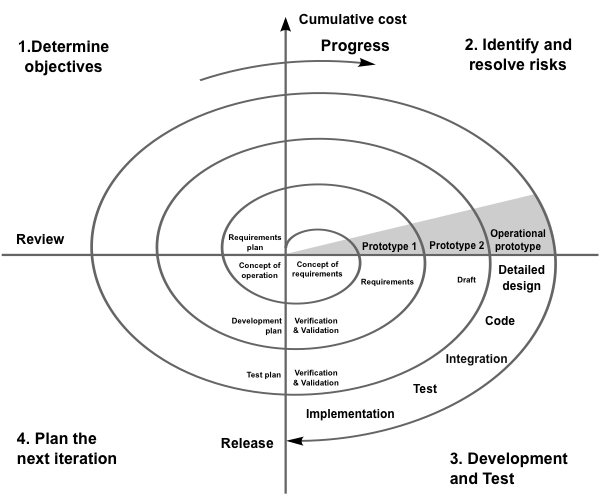
\includegraphics[width=1\textwidth]{includes/figures/chapter4_spiral_life_cycle_schema.png}  \\[0.5 cm]
\end{center}
\caption{Spiral Life-Cycle Schema}
\label{fig:chapter4_spiral_life_cycle_schema}
\end{figure}



The projects will be divided into six cycles, each of them being a particular milestone:
\begin{enumerate}
	\item \textit{Execution of a hello world}: Phase where the first output from the board can be seen.
	\item \textit{Serial output}: Phase aimed to develop the features necessary for printing characters on the serial output of the board and read from an external device.
	\item \textit{HDMI output}: Phase aimed to develop the features necessary for displaying shapes, texts and images on the screen.
	\item \textit{Serial input}: Phase aimed to develop the features necessary for receiving inputs on the board.
	\item \textit{Context Switching}: Phase aimed to develop the features necessary for allowing the kernel to perform context switching and thread scheduling.
	\item \textit{Command line interface}: Phase aimed to develop the feature necessary to present a command line interface to the user.
\end{enumerate}


